\documentclass{article}
\usepackage{physics}
\usepackage{graphicx}
\usepackage{caption}
\usepackage{amsmath}
\usepackage{authblk}
\usepackage{amsfonts}
\usepackage{esint}
\usepackage{mathtools}
\usepackage{amsthm}
\theoremstyle{definition}
\newtheorem{defn}{Definition}[section]
\newtheorem{prop}{Proposition}[section]
\newtheorem{rmk}{Remark}[section]
\newtheorem{exmp}{Example}[section]
\usepackage{empheq}
\usepackage{hyperref}
\usepackage{tensor}
\usepackage{xcolor}
\hypersetup{
	colorlinks,
	linkcolor={black!50!black},
	citecolor={blue!50!black},
	urlcolor={blue!80!black}
}

\begin{document}
\begin{titlepage}\centering
 \clearpage
 \title{\textsc{\bf{PARTIAL\\ DIFFERENTIAL EQUATIONS}}\\\smallskip A Quick Guide\\}
 \author{\bigskip Huan Q. Bui}
 \affil{Colby College\\Physics \& Statistics\\Class of 2021\\}
 \date{\today}
 \maketitle
 \thispagestyle{empty}
\end{titlepage}

\subsection*{Preface}
\addcontentsline{toc}{subsection}{Preface}

Greetings,\\

\textit{Partial Differential Equations: A Quick Guide} is based on my lecture notes from MA411: Topics in Differential Equations - Partial Differential Equations with professor Evan Randles at Colby. The contents are somewhat based on Farlow's \textit{Partial Differential Equations for Scientists and Engineers}.\\	

Enjoy!

\newpage
\tableofcontents
\newpage

\section{Overview and Classification}

%\date{Feb 6, 2019}


\subsection{What in the world is a PDE?}
We shall begin with what PDEs are. 
\begin{defn}
	A partial differential equation (PDE) is an equation relating a function of several variables $\psi(t,\vec{x})$ to its partial derivatives: $\partial_{x_1}\psi$, $\partial^2_{x_1x_2}\psi$, etc.\\
	
	A note on notation:
	\begin{align*}
	\frac{\partial^2 \psi}{\partial x_1\,\partial x_2} \equiv \partial^2_{x_1x_2}\psi \equiv \partial_{x_1}\partial_{x_2}\psi.
	\end{align*}
\end{defn}

\subsection{Some notable examples}
Let us look at a couple of famous PDEs:
\begin{exmp}
	\textbf{Laplace Equation:}
	\begin{align*}
	\Delta \psi = \nabla^2\psi = \frac{\partial^2 \psi}{\partial x^2} + \frac{\partial^2 \psi}{\partial y^2} + \frac{\partial^2 \psi}{\partial z^2} = 0.
	\end{align*}
\end{exmp}

\begin{exmp}
	\textbf{Poisson's Equation:}
	\begin{align*}
	\Delta \psi = \nabla^2 \psi = F(x,y,z)
	\end{align*}
\end{exmp}

We take note of the \textbf{Laplacian} or the \textbf{Laplacian operator}:
\begin{align*}
\boxed{\Delta \psi \equiv \nabla^2 \psi = \frac{\partial^2 \psi}{\partial x^2} + \frac{\partial^2 \psi}{\partial y^2} + \frac{\partial^2 \psi}{\partial z^2}}
\end{align*}
The Laplacian operator takes a function $\psi$ linearly to another function $\nabla^2 \psi$. The Laplacian is one of the most important objects in mathematics, as it touches probability theory, potential theory, partial differential equations, mathematical physics, harmonic analysis, number theory, etc.\\

Another note on notation: the symbols $\Delta$ and $\nabla^2$ will be used interchangeably in this text. The $\nabla^2$ represents the divergence of the gradient.\\

Let us look at some more examples to see the ubiquity of the Laplacian in PDEs:
\begin{exmp}
	\textbf{The heat equation:}
	\begin{align*}
	\frac{\partial \psi}{\partial t} = \nabla^2 \psi.
	\end{align*}
	The heat equation describes heat transfer over time. But there is also a connection between the heat equation and probability theory. In particular, the Gaussian function:
	\begin{align*}
	\frac{1}{\sqrt{4\pi t}}e^{-\frac{x^2}{4t}}
	\end{align*}
	solves the heat equation.
\end{exmp}

\begin{exmp}
	\textbf{The wave equation:}
	\begin{align*}
	\frac{\partial^2 \psi}{\partial t^2} = \nabla^2 \psi.
	\end{align*}
	The wave equation describes physical vibrations. The second $t$-derivative in the equation is strongly correlated to Newton's second law of motion.
\end{exmp}

\begin{exmp}
	\textbf{The Schr\"{o}dinger equation:}
	\begin{align*}
	i\hbar \frac{\partial \psi}{\partial t} = -\frac{\hbar^2}{2m}\nabla^2\psi + V(t,\vec{x})\psi.
	\end{align*}
	One can hardly talk about PDEs without mentioning the Schr\"{o}dinger equation. There is a strong resemblance between the Schr\"{o}dinger equation and the wave equation. Of course, this is no coincidence, as the Schr\"{o}dinger equation is postulated based on a description of a harmonic oscillator.  
\end{exmp}

Our next example does not include the Laplacian operator. 

\begin{exmp}
	\textbf{The telegraphic equation:}
	\begin{align*}
	\frac{\partial^2 \psi}{\partial t^2} = \frac{\partial^2 \psi}{\partial x^2} + \alpha \frac{\partial \psi}{\partial t} + \beta \psi.
	\end{align*}
	The telegraphic equation describes the transfer of information. 
\end{exmp}

\subsection{Vocabulary}
\begin{itemize}
	\item The function $\psi$ appearing in a given PDE is called the ``dependent variable.''
	\item The variables $t,x_1,x_2,\dots$ are called ``independent variables.''
\end{itemize}

\subsection{Our goals}
Our goal is, given a PDE, to find a sufficiently differentiable function which satisfies it that is subject to \textbf{boundary} and \textbf{initial} conditions. 

\subsection{Our plan}
Here are the key concepts we will explore in this text:
\begin{itemize}
	\item Modeling: Formulate same physical problem in terms of PDEs.
	\item Learn how to solve (some) PDEs, subjection to initial conditions and boundary conditions. This means we will be looking at ideas like:
	\begin{itemize}
		\item Separation of variables, in order to reduce a PDE into a system of ODEs.
		\item Integral transforms, in order to reduce the number of independent variables.
		\item Change of coordinates, in order to change a complicated PDE into another one which is easier to solve.
		\item Eigenfunction expansion, which generally goes under the Sturm-Liouville theory.
		\item Numerical methods, as most PDEs cannot be solved analytically. 
	\end{itemize}
\end{itemize}

\subsection{Classification}
\begin{itemize}
	\item The order of a PDE is the highest order of partial derivatives appearing (non-trivially) in the PDE.
	\begin{exmp}
		\begin{align*}
		\frac{\partial \psi}{\partial t} = \nabla^2\psi
		\end{align*}
		is a second-order PDE.
	\end{exmp}
	\begin{exmp}
		\begin{align*}
		\frac{\partial \psi}{\partial t} = \partial^4_x\psi
		\end{align*}
		- the biharmonic heat equation, is a fourth-order PDE.
	\end{exmp}
	\item Linearity: A PDE is linear if the function $\psi$ and its derivatives appear in a linear way.
	\begin{exmp}
		All second-order linear PDEs in 2 variables are of the form:
		\begin{align*}
		\boxed{A\frac{\partial^2 \psi}{\partial x^2} + B\frac{\partial^2 \psi}{\partial x\,\partial y} + C\frac{\partial^2 \psi}{\partial y^2} + D\frac{\partial \psi}{\partial x} + E\frac{\partial \psi}{\partial y} + F\psi = G}
		\end{align*}
	\end{exmp}
\end{itemize}

% Feb 08, 2019

Note: define
\begin{align*}
L[\psi](x,y) = A\frac{\partial^2 \psi}{\partial x^2} + B\frac{\partial^2 \psi}{\partial x\,\partial y} + C\frac{\partial^2 \psi}{\partial y^2} + D\frac{\partial \psi}{\partial x} + E\frac{\partial \psi}{\partial y} + F\psi
\end{align*}
then we get
\begin{align*}
L[u] = G.
\end{align*}
We get a linear map $L:\psi\rightarrow L[\psi]$. So, for $\gamma, \sigma \in \mathbb{R}$
\begin{align*}
L[\gamma u+ \sigma v)] = \gamma L[u] + \sigma L[v].
\end{align*}
This observation justifies the moniker ``linear.'' Next, we say that $L[\psi] = G$ is \textbf{homogeneous} if $G = 0$. The equation is \textbf{inhomogenous} if $G(x,y)\neq 0$ for some $x,y$.\\

If $A,B,C,D,E,F$ are constants, then $L[\psi] = G$ is said to be a \textbf{constant-coefficient} equation. Otherwise (at least one of $A,B,C,D,E,F$ is a function of $x,y$ in some non-trivial way), it is said to have \textbf{variable coefficients}. 

\begin{exmp}
	Classify: $u_t = \sin t u_{xx}$.\\
	
	It is a linear PDE, $A = \sin t$, $B=C=D=F=0$, $E=-1$, $G=0$, variable coefficient, and homogeneous. 
\end{exmp}
\begin{exmp}
	Classify: $u_{xx} -\sin u = 0$.\\
	
	Not linear.
\end{exmp}

\begin{exmp}
	Classify: $xu_x - yu_y = 0$.\\
	
	First-order homogeneous linear PDE with variable coefficients. 
\end{exmp}

Note: Linear PDEs are quite well understood. Notable mathematicians who established theories of linear PDEs: Ehenpres(?), Hille, Browder, Soboher, Nash, Nierenburd, Friedmann, Schwartz, Hormander (Fields, 1962), Gardiy.\\

Note: Constant coefficient equations are \textbf{much easier} to solve than variable coefficient equations, because Fourier analysis makes a lot of the constant coefficient problems easy.\\

Note: Non-linear equations are really hard, and there is no general theory. Each type of non-linear problem demands its own special techniques (well, if they exist at all). 

\subsection{Types of second order linear PDE}
\textbf{Parabolic:} $L[\psi] = G$ is said to be parabolic if $B^2 - 4AC = 0$ ($A,B,C$ don't have to be constant coefficients - so the PDE can be parabolic in some region and not elsewhere). 
\begin{exmp}
	The heat equation
	\begin{align*}
	u_t = u_{xx}
	\end{align*}
	is a parabolic equation, because $A=1, E=-1, B=C=0$. 
\end{exmp}

\textbf{Elliptic:} $L[\psi] = G$ is elliptic if $B^2 - 4AC < 0$.
\begin{exmp}
	Laplace's equation
	\begin{align*}
	\delta u = u_{xx} + u_{yy} = 0
	\end{align*}
	is elliptic, because $A=C=1, B=0$.
\end{exmp}

\textbf{Hyperbolic: } if $B^2 - 4AC > 0$.
\begin{exmp}
	The wave equation:\begin{align*}
	u_{tt} = u_{xx}
	\end{align*}
	is hyperbolic, because $B=0, A=1, C=-1$.
\end{exmp}

\newpage


\section{Diffusion-type problems: A study of the heat equation}
\subsection{An experiment}
We consider a copper rod of length $L$, which allows heat to transfer along the rod, but is insulated in such a way that heat does not transfer laterally across/out of the rod. 
\begin{figure}[h!]
	\centering
	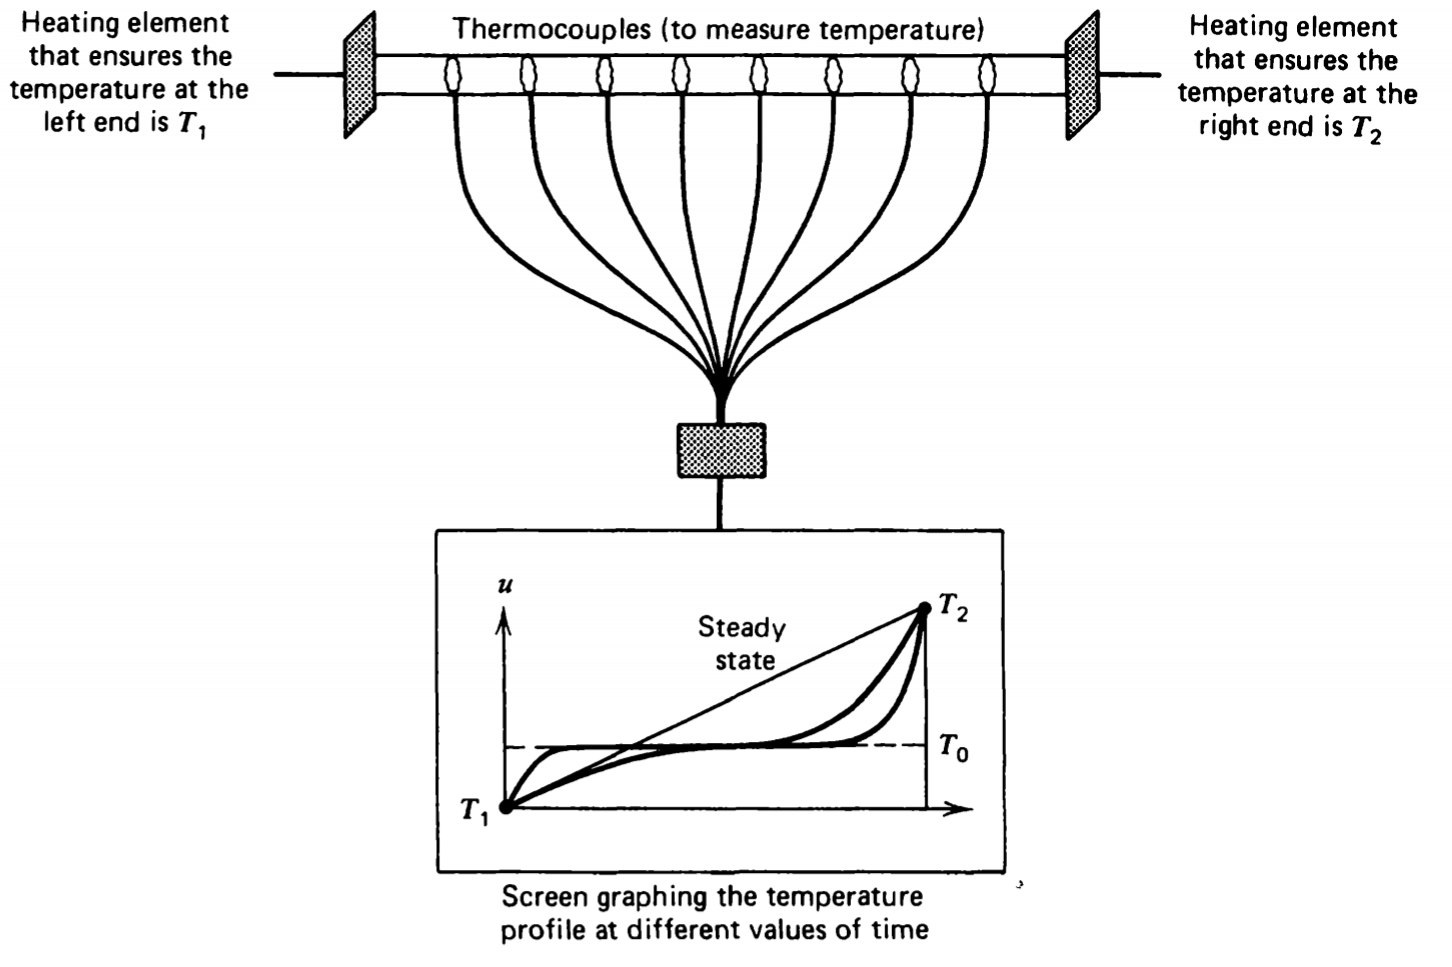
\includegraphics[scale=0.5]{copper.png}
\end{figure}

At time $t=0$, the temperature in the rod is known.
\begin{align*}
u(0,x) = T_0
\end{align*}
The ends of the rod are placed in thermal baths which hold their temperatures fixed. So, at $x=0$, $u(t,0) = T_1$ and at $x=L$, $u(t,L) = T_2$ for all $t>0$. \\

This behavior is modeled by the heat equation. 
\begin{align*}
u_t = \alpha^2 u_{xx},
\end{align*}
where $\alpha \in \mathbb{R}$, determined by the thermo-character of the rod. $u_t$ is the rate of change of temperature in time, and $u_{xx}$ is the concavity profile in space. \\

Some justification for the heat equation: we look at the spatial difference quotient. For small change in $x$, $\Delta x$:
\begin{align*}
u_{xx} &\approx \frac{u_x(t,x+\Delta x) - u_x(t,x)}{\Delta x}\\
&\approx \frac{(u(t,x+\Delta x) - u(t,x))/\Delta x - (u(t,x)-u(t,x-\Delta x))/\Delta x}{\Delta x}\\
&\approx \frac{1}{\Delta x^2}(u(t,x+\Delta x) + u(t,x-\Delta x) - 2u(t,x))\\
&\approx \frac{2}{\Delta x^2}\left(\frac{u(t,x+\Delta x) + u(t,x-\Delta x)}{2} - u(t,x) \right)
\end{align*}
So, $u_{xx} \propto$ the difference between the average temperatures among neighboring points and the temperature at $x$. 
\begin{figure}[h!]
	\centering
	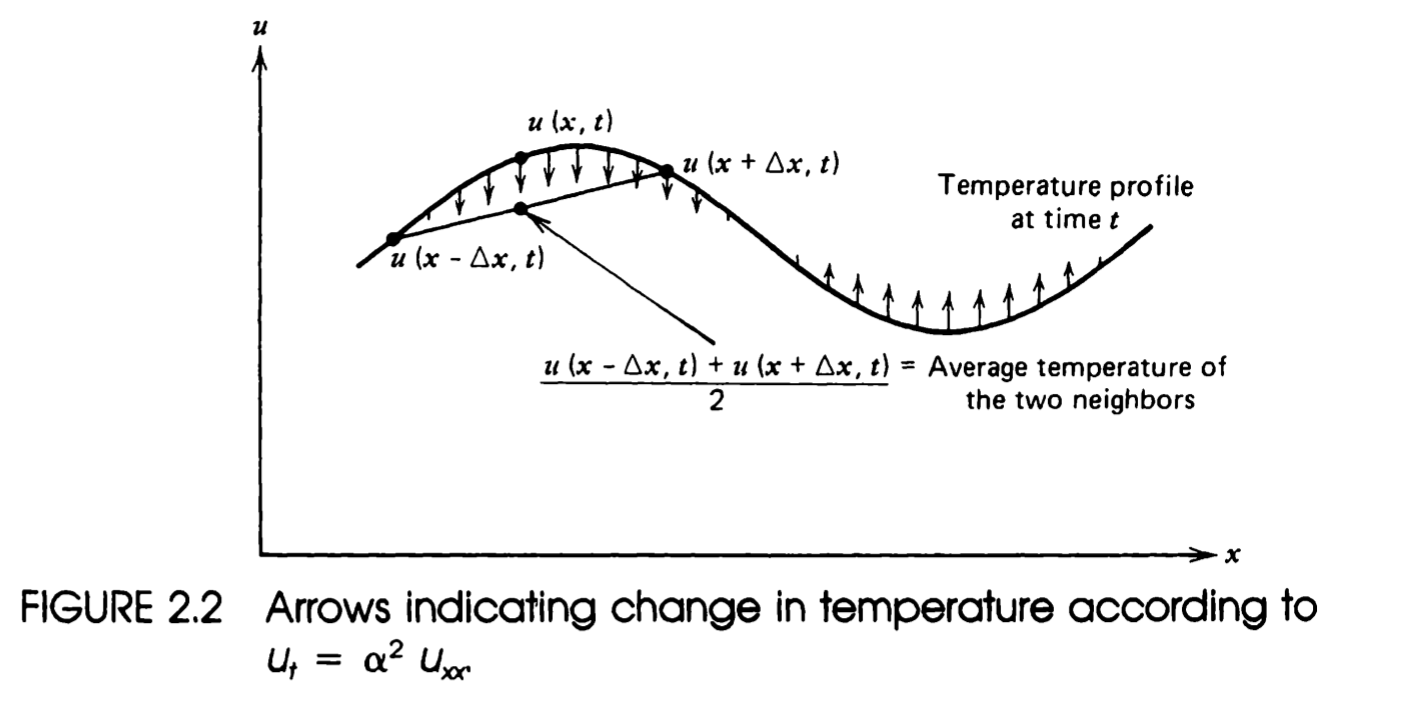
\includegraphics[scale=0.5]{copper1.png}
\end{figure}

Assume that $u_t = \alpha^2 u_{xx}$, then if $u_{xx} < 0$, then $u_t < 0$, i.e. temperature decreases in time. If $u_{xx} > 0$, then $u_t > 0$, i.e. temperature increases in time. If $u_{xx} = 0$, the temperature stays fixed. 

\end{document}
